No requieren de un medio para propagarse. Por tanto, pueden viajar haya o no un medio presente.

Están formadas por campos magnéticos y eléctricos que oscilan perpendicularmente entre sí y a la dirección de propagación. Debido a esto, este tipo de onda es siempre \transversal.

\begin{figure}[H]
  \centering
  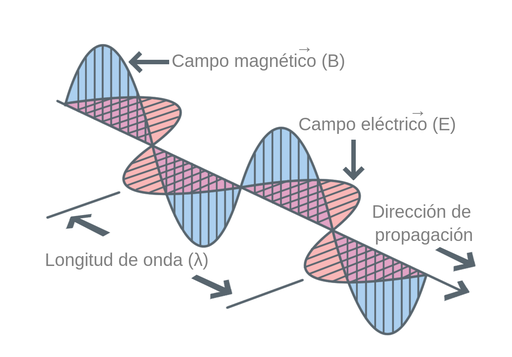
\includegraphics[scale=0.5]{imagenes/campo_electrico_magnetico.png}
  \caption{Vectores de campo eléctrico y magnético oscilantes\cite{labstercampoelcmag}}
\end{figure}

El rango completo de radiación electromagnética se conoce como \EspectroElectromagnetico.
